\documentclass{vkr}
\usepackage[english, russian]{babel} % переносы
\usepackage{graphicx} % для вставки картинок
\graphicspath{{images/}} % путь к изображениям
\usepackage[hidelinks]{hyperref}
\usepackage{float} % определяет метод H для рисунка с переносом на следующую страницу, ели не помещается
\usepackage{pdflscape}
\addto{\captionsrussian}{\renewcommand{\refname}{СПИСОК ИСПОЛЬЗОВАННЫХ ИСТОЧНИКОВ}}
\usepackage{xltabular} % для вставки таблиц
\usepackage{makecell}
\renewcommand\theadfont{} % шрифт в /thead
\usepackage{array} % для определения новых типов столбцов таблиц
\newcolumntype{T}{>{\centering\arraybackslash}X} % новый тип столбца T - автоматическая ширина столбца с выравниванием по центру
\newcolumntype{R}{>{\raggedleft\arraybackslash}X} % новый тип столбца R - автоматическая ширина столбца с выравниванием по правому краю
\newcolumntype{C}[1]{>{\centering\let\newline\\\arraybackslash\hspace{0pt}}m{#1}} % новый тип столбца C - фиксированная ширина столбца с выравниванием по центру
\newcolumntype{r}[1]{>{\raggedleft\arraybackslash}p{#1}} % новый тип столбца r - фиксированная ширина столбца с выравниванием по правому краю
\newcommand{\centrow}{\centering\arraybackslash} % командой \centrow можно центрировать одну ячейку (заголовок) в столбце типа X или p, оставив в оcтальных ячейках другой тип выравнивания
\newcommand{\finishhead}{\endhead\hline\endlastfoot}
\newcommand{\continuecaption}[1]{\caption*{#1}\\ \hline }
\usepackage{etoolbox}
\AtBeginEnvironment{xltabular}{\refstepcounter{tablecnt}} % подсчет таблиц xltabular, обычные таблицы подсчитываются в классе

\usepackage[tableposition=top]{caption} % подпись таблицы вверху
\captionsetup{strut=off}
\setlength{\intextsep}{0pt} % Vertical space above & below [h] floats
\setlength{\textfloatsep}{0pt} % Vertical space below (above) [t] ([b]) floats
\DeclareCaptionLabelFormat{gostfigure}{Рисунок #2} %подпись рисунка
\DeclareCaptionLabelFormat{gosttable}{Таблица #2} %подпись таблицы
\DeclareCaptionLabelSeparator{gost}{~--~} %разделитель в рисунках и таблицах
\captionsetup{labelsep=gost}
\captionsetup[figure]{aboveskip=10pt,belowskip=4mm,justification=centering,labelformat=gostfigure} % настройка подписи рисунка
\captionsetup[table]{font={stretch=1.41},skip=0pt,belowskip=0pt,aboveskip=8.5pt,singlelinecheck=off,labelformat=gosttable} % настройка подписи таблицы

\setlength{\LTpre}{8mm} % отступ сверху таблицы
\setlength{\LTpost}{6mm} % отступ снизу таблицы

\usepackage{enumitem}
\setlist{nolistsep,wide=\parindent,itemindent=*} % отступы вокруг списков, выравнивание с учетом разделителя

\usepackage{color} %% это для отображения цвета в коде
\usepackage{listings} %% листинги кода
\setmonofont[Scale=0.7]{Verdana} % моноширный шрифт для листинга

\definecolor{codegreen}{rgb}{0,0.6,0}
\definecolor{codegray}{rgb}{0.5,0.5,0.5}
\definecolor{codepurple}{rgb}{0.58,0,0.82}

\lstset{ %
language=C,                 % выбор языка для подсветки (здесь это С)
numbers=left,               % где поставить нумерацию строк (слева\справа)
numberstyle=\tiny,           % размер шрифта для номеров строк
stepnumber=1,                   % размер шага между двумя номерами строк
numbersep=5pt,                % как далеко отстоят номера строк от подсвечиваемого кода
commentstyle=\color{codegreen},
keywordstyle=\color{magenta},
numberstyle=\tiny\color{codegray},
stringstyle=\color{codepurple},
basicstyle=\linespread{0.95}\ttfamily,
backgroundcolor=\color{white}, % цвет фона подсветки - используем \usepackage{color}
showspaces=false,            % показывать или нет пробелы специальными отступами
showstringspaces=false,      % показывать или нет пробелы в строках
showtabs=false,             % показывать или нет табуляцию в строках
frame=single,              % рисовать рамку вокруг кода
tabsize=2,                 % размер табуляции по умолчанию равен 2 пробелам
captionpos=t,              % позиция заголовка вверху [t] или внизу [b] 
breaklines=true,           % автоматически переносить строки (да\нет)
breakatwhitespace=false, % переносить строки только если есть пробел
escapeinside={\%*}{*)}   % если нужно добавить комментарии в коде
}

\makeatletter % чтобы допускались русские комментарии в листингах
\lst@InputCatcodes
\def\lst@DefEC{%
 \lst@CCECUse \lst@ProcessLetter
  ^^80^^81^^82^^83^^84^^85^^86^^87^^88^^89^^8a^^8b^^8c^^8d^^8e^^8f%
  ^^90^^91^^92^^93^^94^^95^^96^^97^^98^^99^^9a^^9b^^9c^^9d^^9e^^9f%
  ^^a0^^a1^^a2^^a3^^a4^^a5^^a6^^a7^^a8^^a9^^aa^^ab^^ac^^ad^^ae^^af%
  ^^b0^^b1^^b2^^b3^^b4^^b5^^b6^^b7^^b8^^b9^^ba^^bb^^bc^^bd^^be^^bf%
  ^^c0^^c1^^c2^^c3^^c4^^c5^^c6^^c7^^c8^^c9^^ca^^cb^^cc^^cd^^ce^^cf%
  ^^d0^^d1^^d2^^d3^^d4^^d5^^d6^^d7^^d8^^d9^^da^^db^^dc^^dd^^de^^df%
  ^^e0^^e1^^e2^^e3^^e4^^e5^^e6^^e7^^e8^^e9^^ea^^eb^^ec^^ed^^ee^^ef%
  ^^f0^^f1^^f2^^f3^^f4^^f5^^f6^^f7^^f8^^f9^^fa^^fb^^fc^^fd^^fe^^ff%
  ^^^^20ac^^^^0153^^^^0152%
  % Basic Cyrillic alphabet coverage
  ^^^^0410^^^^0411^^^^0412^^^^0413^^^^0414^^^^0415^^^^0416^^^^0417%
  ^^^^0418^^^^0419^^^^041a^^^^041b^^^^041c^^^^041d^^^^041e^^^^041f%
  ^^^^0420^^^^0421^^^^0422^^^^0423^^^^0424^^^^0425^^^^0426^^^^0427%
  ^^^^0428^^^^0429^^^^042a^^^^042b^^^^042c^^^^042d^^^^042e^^^^042f%
  ^^^^0430^^^^0431^^^^0432^^^^0433^^^^0434^^^^0435^^^^0436^^^^0437%
  ^^^^0438^^^^0439^^^^043a^^^^043b^^^^043c^^^^043d^^^^043e^^^^043f%
  ^^^^0440^^^^0441^^^^0442^^^^0443^^^^0444^^^^0445^^^^0446^^^^0447%
  ^^^^0448^^^^0449^^^^044a^^^^044b^^^^044c^^^^044d^^^^044e^^^^044f%
  ^^^^0401^^^^0451%
  %%%
  ^^00}
\lst@RestoreCatcodes
\makeatother


% Режим шаблона (должен быть включен один из трех)
%\ВКРtrue
\Практикаtrue
%\Курсоваяtrue

\newcommand{\Дисциплина}{<<Проектирование и архитектура программных систем>>} % для курсовой
\newcommand{\КодСпециальности}{09.03.04} % Курсовая
\newcommand{\Специальность}{Программная инженерия} % Курсовая
\newcommand{\Тема}{Разработка web-сайта «Русатом – Аддитивные технологии» на платформе} % ВКР Курсовая
\newcommand{\ТемаВтораяСтрока}{1С-Битрикс}
\newcommand{\ГдеПроводитсяПрактика}{Юго-Западном государственном университете} % для практики
\newcommand{\РуководительПрактПредпр}{} % для практики
\newcommand{\ДолжнРуководительПрактПредпр}{директор} % для практики
\newcommand{\РуководительПрактУнивер}{Чаплыгин А. А.} % для практики
\newcommand{\ДолжнРуководительПрактУнивер}{к.т.н. доцент} % для практики
\newcommand{\Автор}{И. И. Иванов}
\newcommand{\АвторРод}{Иванова И.И.}
\newcommand{\АвторПолностьюРод}{Яременко Максима Владимировича} % для практики
\newcommand{\Шифр}{хх-хх-хххх}
\newcommand{\Курс}{4} % для практики
\newcommand{\Группа}{ПО-02б}
\newcommand{\Руководитель}{А. А. Чаплыгин} % для ВКР и курсовой
\newcommand{\Нормоконтроль}{А. А. Чаплыгин} % для ВКР
\newcommand{\ЗавКаф}{А. В. Малышев} % для ВКР
\newcommand{\ДатаПриказа}{«07» апреля 2023~г.} % для ВКР
\newcommand{\НомерПриказа}{1505-с} % для ВКР
\newcommand{\СрокПредоставления}{«13» июня 2023~г.} % для ВКР, курсового

\begin{document}
\maketitle
\ifПрактика{}\else{
   \newpage
\begin{center}
\large\textbf{Минобрнауки России}

\large\textbf{Юго-Западный государственный университет}
\vskip 1em
\normalsize{Кафедра программной инженерии}
\vskip 1em
\ifВКР{
        \begin{flushright}
        \begin{tabular}{p{.4\textwidth}}
        \centrow УТВЕРЖДАЮ: \\
        \centrow Заведующий кафедрой \\
        \hrulefill \\
        \setarstrut{\footnotesize}
        \centrow\footnotesize{(подпись, инициалы, фамилия)}\\
        \restorearstrut
        «\underline{\hspace{1cm}}»
        \underline{\hspace{3cm}}
        20\underline{\hspace{1cm}} г.\\
        \end{tabular}
        \end{flushright}
        }\fi
\end{center}
\vspace{1em}
  \begin{center}
  \large
\ifВКР{
ЗАДАНИЕ НА ВЫПУСКНУЮ КВАЛИФИКАЦИОННУЮ РАБОТУ
  ПО ПРОГРАММЕ БАКАЛАВРИАТА}
  \else
ЗАДАНИЕ НА КУРСОВУЮ РАБОТУ (ПРОЕКТ)
\fi
\normalsize
  \end{center}
\vspace{1em}
{\parindent0pt
  Студента \АвторРод, шифр\ \Шифр, группа \Группа
  
1. Тема «\Тема\ \ТемаВтораяСтрока»
\ifВКР{
утверждена приказом ректора ЮЗГУ от \ДатаПриказа\ № \НомерПриказа
}\fi.

2. Срок предоставления работы к защите \СрокПредоставления

3. Исходные данные для создания программной системы:

3.1. Перечень решаемых задач:}

\renewcommand\labelenumi{\theenumi)}

\begin{enumerate}
\item Анализ существующих игр-платформеров.
\item Разработка концептуальной модели игр-платформеров.
\item Проектирование программной системы для создания игр-платформеров.
\item Реализация программной системы для создания игр-платформеров.
\item Тестирование разработанной системы.
\end{enumerate}

{\parindent0pt
  3.2. Входные данные и требуемые результаты для программы:}

\begin{enumerate}
\item Входными данными для программной системы являются: данные  конфигураций, ПО, критериев качества SLA,
ИТ-услуг, информация о языке Python, спрайтовые изображения.
\item Выходными данными для программной системы являются: приложение для разработки компьютерных игр-платформеров.
\end{enumerate}

{\parindent0pt

  4. Содержание работы (по разделам):
  
  4.1. Введение
  
  4.1. Анализ предметной области
  
4.2. Техническое задание: основание для разработки, назначение разработки,
требования к программной системе, требования к оформлению документации.

4.3. Технический проект: общие сведения о программной системе, проект
данных программной системы, проектирование архитектуры программной системы, проектирование пользовательского интерфейса программной системы.

4.4. Рабочий проект: спецификация компонентов и классов программной системы, тестирование программной системы, сборка компонентов программной системы.

4.5. Заключение

4.6. Список использованных источников

5. Перечень графического материала:

\списокПлакатов

\vskip 2em
\begin{tabular}{p{6.8cm}C{3.8cm}C{4.8cm}}
Руководитель \ifВКР{ВКР}\else работы (проекта) \fi & \lhrulefill{\fill} & \fillcenter\Руководитель\\
\setarstrut{\footnotesize}
& \footnotesize{(подпись, дата)} & \footnotesize{(инициалы, фамилия)}\\
\restorearstrut
Задание принял к исполнению & \lhrulefill{\fill} & \fillcenter\Автор\\
\setarstrut{\footnotesize}
& \footnotesize{(подпись, дата)} & \footnotesize{(инициалы, фамилия)}\\
\restorearstrut
\end{tabular}
}

\renewcommand\labelenumi{\theenumi.}

   \abstract{РЕФЕРАТ}

Объем работы равен \formbytotal{lastpage}{страниц}{е}{ам}{ам}. Работа содержит \formbytotal{figurecnt}{иллюстраци}{ю}{и}{й}, \formbytotal{tablecnt}{таблиц}{у}{ы}{}, \arabic{bibcount} библиографических источников и \formbytotal{числоПлакатов}{лист}{}{а}{ов} графического материала. Количество приложений – 2. Графический материал представлен в приложении А. Фрагменты исходного кода представлены в приложении Б.

Перечень ключевых слов: коммерческий сайт, Система, CMS, Битрикс, Joomla, аддитивные технологии, 3D-принтеры, услуги, сервисы, информатизация, автоматизация, информационные технологии, веб-форма,  Apache, классы, база данных, средства защиты информации, подсистема, компонент, модуль, сущность, информационный блок, метод, контент-редактор, администратор, пользователь, web-сайт.

Объектом разработки является web-сайт компании,  занимающейся производством 3D-принтеров, выпуском оборудования для создания порошков, разработкой программного обеспечения и организацией центров аддитивного производства.

Целью выпускной квалификационной работы является привлечение клиентов, увеличение заказов, информирование о продукции и услугах путем создания сайта компании.

В процессе создания сайта были выделены основные сущности путем создания информационных блоков, использованы классы и методы модулей, обеспечивающие работу с сущностями предметной области, а также корректную работу web-сайта, разработаны разделы, содержащие информацию о компании, ее деятельности, производимой продукции и услугах, разработан сервис по заказу 3D-деталей.

При разработке сайта использовалась система управления контентом "<1С-Битрикс: Управление сайтом">.

Разработанный сайт был успешно внедрен в компании.

\selectlanguage{english}
\abstract{ABSTRACT}
  
The volume of work is \formbytotal{lastpage}{page}{}{s}{s}. The work contains \formbytotal{figurecnt}{illustration}{}{s}{s}, \formbytotal{tablecnt}{table}{}{s}{s}, \arabic{bibcount} bibliographic sources and \formbytotal{числоПлакатов}{sheet}{}{s}{s} of graphic material. The number of applications is 2. The graphic material is presented in annex A. The layout of the site, including the connection of components, is presented in annex B.

List of keywords: commercial website, System, CMS, Bitrix, Joomla, additive technologies, 3D printers, services, services, informatization, automation, information technology, web form, Apache, classes, database, component, module, entity, information block, method, content editor, administrator, user, web site.

The object of the research is the analysis of information technologies for the development of a production company's website.

The object of the development is the website of a company engaged in the production of 3D printers, the production of equipment for the creation of powders, software development and the organization of additive manufacturing centers.

The purpose of the final qualifying work is to attract customers, increase orders, inform about products and services by creating a company website.

In the process of creating the site, the main entities were identified by creating information blocks, classes and methods of modules were used to ensure work with the entities of the subject area, as well as the correct operation of the website, sections containing information about the company, its activities, products and services were developed, a service for ordering 3D parts was developed.

When developing the site, the content management system <<1C – Bitrix: Site Management>> was used.

The developed website was successfully implemented in the company.
\selectlanguage{russian}
}\fi
\tableofcontents
\section*{ОБОЗНАЧЕНИЯ И СОКРАЩЕНИЯ}

ИС -- информационная система.

ИТ -- информационные технологии. 

КТС -- комплекс технических средств.

ПО -- программное обеспечение.

РП -- рабочий проект.

ТЗ -- техническое задание.

ТП -- технический проект.

\ifПрактика{}\else{\section*{ВВЕДЕНИЕ}
\addcontentsline{toc}{section}{ВВЕДЕНИЕ}

С развитием цифровых технологий и увеличением вычислительной мощности персональных компьютеров, появилась возможность создания сложных и многофункциональных программных продуктов, в том числе и для развлекательной индустрии. Одним из таких направлений является разработка игр-платформеров, которые погружают пользователя в новые виртуальные вселенные с заранее отрисованными фонами и спрайтами. Эти элементы игры не только создают уникальную атмосферу и мир, но и являются ключевыми компонентами в структуре игрового процесса.

Как и аддитивные технологии, которые кардинально изменили подход к проектированию и производству, программные системы для создания игр-платформеров представляют собой инновационный инструмент, который позволяет разработчикам с минимальными затратами времени и ресурсов создавать захватывающие игры. Это стало возможным благодаря использованию специальных библиотек (например:Pygame), готовых ассетов, таких как фоны и спрайты, а также благодаря гибким инструментам для их интеграции и анимации.

Таким образом, программные системы для создания игр-платформеров с заранее отрисованным фоном и спрайтами являются частью более широкого тренда цифровизации и автоматизации, который охватывает многие отрасли, включая развлекательную индустрию. Они позволяют разработчикам сосредоточиться на творческом процессе, минимизируя технические аспекты реализации проекта.

\emph{Цель настоящей работы} – разработка приложения для разработки игр платформеров с заранее отрисованными спрайтами и фоном. Для достижения поставленной цели необходимо решить следующие задачи:
\begin{itemize}
	\item провести анализ предметной области;
	\item разработать концептуальную модель приложения;
	\item спроектировать приложение;
	\item реализовать приложение средствами языка программирования python.
\end{itemize}


\emph{Структура и объем работы.} Отчет состоит из введения, 4 разделов основной части, заключения, списка использованных источников, 2 приложений. Текст выпускной квалификационной работы равен \formbytotal{page}{страниц}{е}{ам}{ам}.

\emph{Во введении} сформулирована цель работы, поставлены задачи разработки, описана структура работы, приведено краткое содержание каждого из разделов.

\emph{В первом разделе} на стадии описания технической характеристики предметной области приводится сбор информации о деятельности компании, для которой осуществляется разработка сайта.

\emph{Во втором разделе} на стадии технического задания приводятся требования к разрабатываемой программной системе.

\emph{В третьем разделе} на стадии технического проектирования представлены проектные решения для программной системы.

\emph{В четвертом разделе} приводится список классов и их методов, использованных при разработке программной системы, производится тестирование разработанной программной системы.

В заключении излагаются основные результаты работы, полученные в ходе разработки.

В приложении А представлен графический материал.
В приложении Б представлены фрагменты исходного кода. 
}\fi
\section{Анализ предметной области}
\subsection{История и описание игр-платформеров}

Платфо́рмер (англ. platformer, platform game) — жанр компьютерных игр, в которых основу игрового процесса составляют прыжки по платформам, лазанье по лестницам, сбор предметов, необходимых для победы над врагами или завершения уровня.Многие игры подобного жанра характеризуются нереалистичностью, рисованной мультяшной графикой. Персонажами таких игр часто бывают вымышленные существа (к примеру, драконы, гоблины) или антропоморфные животные.
Платформеры появились в начале 1980-х и стали трёхмерными ближе к концу 1990-х. Через некоторое время после образования жанра у него появилось данное название, отражающее тот факт, что в платформерах геймплей сфокусирован на прыжках по платформам в противовес стрельбе. Правда, во многих платформерах присутствует стрелковое оружие, в таких, например, как Blackthorne или Castlevania. Последняя послужила основой поджанра метроидвания. 

Некоторые предметы, называемые пауэр-апами (англ. power-up), наделяют управляемого игроком персонажа особой силой, которая обычно иссякает со временем (к примеру: силовое поле, ускорение, увеличение высоты прыжков). Коллекционные предметы, оружие и «пауэр-ап» собираются обычно простым прикосновением персонажа и для применения не требуют специальных действий со стороны игрока. Реже предметы собираются в «инвентарь» героя и применяются специальной командой (такое поведение более характерно для аркадных головоломок). Сходный жанр компьютерных игр сайд-скроллер.

Противники (называемые «врагами»), всегда многочисленные и разнородные, обладают примитивным искусственным интеллектом, стремясь максимально приблизиться к игроку, либо не обладают им вовсе, перемещаясь по круговой дистанции или совершая повторяющиеся действия. Соприкосновение с противником обычно отнимает жизненные силы у героя или вовсе убивает его. Иногда противник может быть нейтрализован либо прыжком ему на голову, либо из оружия, если им обладает герой. Смерть живых существ обычно изображается упрощённо или символически (существо исчезает или проваливается вниз за пределы экрана).

Уровни, как правило, изобилуют секретами (скрытые проходы в стенах, высокие или труднодоступные места), нахождение которых существенно облегчает прохождение и подогревает интерес игрока.
\subsection{История жанра}
Платформеры появились в начале 1980-х, когда игровые консоли не были достаточно мощными, чтобы отображать трёхмерную графику или видео. Они были ограничены статическими игровыми мирами, которые помещались на один экран, а игровой герой был виден в профиль. Персонаж лазал вверх и вниз по лестницам или прыгал с платформы на платформу, часто сражаясь с противниками и собирая предметы, улучшающие характеристики (так называемые «пауэрапы»). Первыми играми этого типа были Space Panic и Apple Panic. За ними последовала игра Donkey Kong, аркадная игра созданная фирмой «Nintendo» и выпущенная в 1981 году. Вскоре процесс прохождения уровня перестал быть в основном вертикальным и стал горизонтальным с появлением длинных многоэкранных прокручивающихся игровых миров. Считается, что начало этому положила выпущенная фирмой Activision в 1982 году игра Pitfall! для консолей Atari 2600. Manic Miner (1983) и её продолжение Jet Set Willy (1984) были наиболее популярными платформерами на домашних компьютерах.

В 1985 году фирма «Nintendo» выпустила для приставки Nintendo Entertainment System революционный платформер Super Mario Bros. Игра была наполнена большими и сложными уровнями, и стала примером для последующих создателей игр, и даже сегодня многие люди считают её одной из самых лучших видеоигр. Игра имела фантастическую популярность и продавалась огромными тиражами. Для многих людей она стала первым в их жизни платформером, а главный герой Марио стал символом фирмы «Nintendo».

Термин «трёхмерный платформер» может обозначать или геймплей, включающий все три измерения, или использование трёхмерных полигонов в реальном времени для отрисовки уровней и героев, или и то и другое. Появление трёхмерных платформеров принесло изменение конечных целей некоторых платформеров. В большинстве двумерных платформеров игроку нужно было достичь на уровне только одной цели, однако во многих трёхмерных платформерах, каждый уровень необходимо прочесывать, собирая кусочки головоломок (Banjo-Kazooie) или звезды (Super Mario 64). Это дало возможность более эффективного использования больших трёхмерных областей и вознаграждало игрока за тщательное исследование уровня, но некоторые игроки считают собирание бесчисленных безделушек более нудным занятием, чем игровые испытания. Donkey Kong 64 была раскритикована за то, что игроку приходилось часто переключаться между пятью различными игровыми героями, чтобы получить бананы различных цветов и другие предметы. Однако не все трёхмерные платформеры были такими, самым ярким примером является Crash Bandicoot. Эта игра оставалось верной традиции двумерных платформеров и в ней использовались довольно плоские уровни, в конце которых располагалась игровая цель.

В 2000-х гг. продолжилось развитие и популяризация 3D-платформеров (Pane. 2016). В 2002 г. была выпущена «Ratchet \& Clank», в которой пользователи наблюдали за игровым процессом как от первого, так и от третьего лица. Также они могли использовать множество видов оружия для борьбы с противниками и преодоления препятствий. В 2005 г. вышла игра «Psychonauts». В процессе прохождения пользователи открывали сверхъестественные психические способности, такие как телекинез, левитация, невидимость и пирокинез. Это позволяло протагонисту исследовать большую часть локаций, а также сражаться с врагами. Иной геймплей был у «Little Big Planet» (2008). В игре, представляющей собой приключенческий платформер, содержались элементы головоломки. Кроме того, пользователям открывалась уникальная возможность редактирования и создания собственных уровней.

В 2010 г. вышла «Super Meat Boy», выполненная в стиле классических 2D-платформеров. В 2015 г. была выпущена «Ori and the Blind Forest», а в 2017 г. «Hollow Knight» и «Cuphead», обладающие уникальным графическим стилем и отличающиеся повышенной сложностью прохождения. В то же время вышли продолжения серий, зародившихся ещё в 1980–1990-х гг. (Pane. 2016). Например, в 2013 г. был выпущен музыкальный 2D-платформер «Rayman Legends», а в 2017 г. «Super Mario Odyssey», выполненный в 3D-графике. Также стали появляться бесконечные платформеры (англ. «endless runner»), предназначенные для мобильных устройств, например, «Temple Run» (2011) и «Jetpack Joyride» (2011). В поздние 2010-е гг. популярность обрели приключенческие платформеры, относящиеся к поджанрам roguelike и метроидвания. К играм данного типа относятся «Dead Cells» 2018 г. и «Blasphemous» 2019 г. Другим направлением развития жанра платформера стали кооперативные 3D-проекты, например «Biped» (2020) и «It Takes Two» (2021).

Как и другие жанры, платформер активно изучают специалисты Game Studies. Особый интерес для учёных представляет игровой опыт пользователей и их восприятие цифровых продуктов. Например функция, которая подразумевает смерть и последующее возрождение подконтрольного персонажа. Данная игровая особенность, свойственная платформерам, тесно связана с формированием впечатлений при ознакомлении пользователей с цифровым продуктом. Так, когда игроки погружены в игровой процесс, риск смерти способен вызвать беспокойство за персонажа. Это побуждает пользователей к взвешенному принятию решений. Сочувствие к персонажу может вызывать сильные эмоции, активизирующиеся при прохождении всё более сложных уровней (Mecler. 2020).

Также учёные исследуют методы создания и совершенствования проектов, например, построение уровней при помощи искусственного интеллекта. К примеру, в 2010 г. команда американских учёных изучала различные подходы генерации уровней 2D-платформеров. Выяснилось, что алгоритм, основанный на ритмах, обеспечивает большую гибкость при создании игровых этапов. Под ритмами понималась комбинация геометрического строения уровня и действий игроков, направленных на прохождение этапа или преодоление возникших препятствий (Launchpad. 2011). Кроме того, учёные рассматривали построение уровней при помощи модульного расширения существующего игрового движка «Unity». Исследователи задействовали структурные (типы и положения платформ) и функциональные (физику и возможности перемещения персонажа) особенности уровней, а также вероятность успеха при совершении одиночных прыжков (Aramini. 2018). В основе такого типа публикаций зачастую лежит статистика игроков, отражающая способы и паттерны прохождения ими уровней.
\section{Техническое задание}
\subsection{Основание для разработки}

Основанием для разработки является задание на выпускную квалификационную работу бакалавра "<Разработка движка \textquotedbl для игр-платформеров">.

\subsection{Цель и назначение разработки}

Основной задачей выпускной квалификационной работы является разработка "движка" игр-платформеров для продвижения их популярности. Данный программный продукт предназначен для демонстрации практических навыков, полученных в течение обучения.

Целью данной разработки является создание движка платформер игры и популяризация этого игрового жанра.

Задачами данной разработки являются:
\begin{itemize}
\item проектирование интерфейса;
\item проектирование игрового сценария;
\item реализация взаимодействия приложения с пользователем;
\item реализация механик игр-платформеров;
\item реализация графики приложения;
\item реализация камеры;
\end{itemize}

\subsection{Требования пользователя к движку}

Движок должен включать в себя:
\begin{itemize}
    \item реализацию основных механик платформера;
    \item реализацию физики платформ и персонажа;
    \item реализация смены сценариев;
    \item реализация передвижения персонажа по уровню;
    \item реализацию камеры.
\end{itemize}



\subsection{Правила игры}
!!!!!!!!!!!!!!Главный герой игры (ГГ) перемещается по уровням собирая различные предметы(усилители) и кольца(очки). Внутри каждого уровня существуют препятствия и враги которых главному герою предстоит преодолеть. Начинается игра с предыстории в виде текста в диалоговой панели, который пользователь должен прочесть. Далее персонаж попадает на первый уровень,который ему надо пройти. Для того, чтобы пройти игру, нужно пройти все уровни. Изначально для прохождения доступен только первый уровень, а по мере прохождения открываются последующие уровни. 
Процесс прохождения уровней заключается в преодолении препятствий,зарабатыванием очков, взаимодействии с усилителями, предметами и локациями игрового мира. Пройдя уровень игрок получает доступ к следующему уровню. Игрок может взаимодействовать с игровым миром с помощью компьютерной мыши и клавиш(Space,Ctrl,Q,E). При получении усилителя игрок может использовать его при помощи клавиши Q,при получении определенного кол-ва очков игрок может получить доп.жизнь клавишей E,перемещение осуществляется автоматически кроме прыжков и подкатов(Space и Ctrl). Доступны следующие объекты взаимодействия с игроком:
\begin{enumerate}
\item Усилитель – при нажатии клавиши Q активирует усилитель. При активации усилителя  придает ГГ ускорение на некоторое время.
\item Кольца – предметы являющиеся обычными очками набираемыми при прохождении. Если у ГГ находится больше 50 колец, при помощи клавиши E можно активировать доп.жизнь.
\item Переход на другую локацию – при наведении иконка курсора меняется на стрелку в направлении доступной локации, в которую хочет перейти пользователь.
\end{enumerate}

\subsection{Сюжет игры}

Главный герой безымянный рыцарь.............................

\subsection{Интерфейс пользователя}

На основании анализа предметной области в программе должны быть реализованы следующие прецеденты:
\begin{enumerate}
	\item Перемещение по уровням;
	\item Графическое отображение уровней;
	\item Взаимодействие с игровыми объектами при помощи компьютерной мыши и клавиш компьютера.
\end{enumerate}

\subsection{Требования к оформлению документации}

Разработка программной документации и программного изделия должна производиться согласно ГОСТ 19.102-77 и ГОСТ 34.601-90. Единая система программной документации.

\section{Технический проект}
\subsection{Общая характеристика организации решения задачи}

Необходимо спроектировать и разработать приложение, который должен способствовать популяризации игр-платформеров.

Приложение представляет собой набор взаимосвязанных различных окон, которые сгруппированы по разделам, содержащие текстовую, графическую информацию. Приложение располагается на компьютере. При разработке используется библиотека Pygame.

\subsection{Обоснование выбора технологии проектирования}

На сегодняшний день информационный рынок, поставляющий программные решения в выбранной сфере, предлагает множество продуктов, позволяющих достигнуть поставленной цели – разработки игрового приложения.

\subsubsection{Описание используемых технологий и языков программирования}

В процессе разработки приложения используются программные средства и языки программирования. Каждое программное средство и каждый язык программирования применяется для круга задач, при решении которых они необходимы.

\subsubsection{Язык программирования Python}

Python –  высокоуровневый язык программирования общего назначения с динамической строгой типизацией и автоматическим управлением памятью, ориентированный на повышение производительности разработчика, читаемости кода и его качества, а также на обеспечение переносимости написанных на нём программ. Язык является полностью объектно-ориентированным в том плане, что всё является объектами. Необычной особенностью языка является выделение блоков кода отступами. Синтаксис ядра языка минималистичен, за счёт чего на практике редко возникает необходимость обращаться к документации. Сам же язык известен как интерпретируемый и используется в том числе для написания скриптов. Недостатками языка являются зачастую более низкая скорость работы и более высокое потребление памяти написанных на нём программ по сравнению с аналогичным кодом, написанным на компилируемых языках, таких как C или C++.

\paragraph{Достоинства языка Python}
\begin{itemize}
	\item Простота и читаемость кода: Python использует простой и чистый синтаксис, что делает код легким для понимания и обслуживания.
	\item Многофункциональность: Python подходит для создания различных типов приложений, включая веб-приложения, настольные приложения, научные вычисления, обработку данных и многое другое
	\item Большой выбор библиотек: Python имеет огромное сообщество разработчиков, что приводит к большому количеству библиотек и модулей для различных задач. Например, для машинного обучения есть библиотека TensorFlow, для веб-разработки - Django, для анализа данных - Pandas и многое другое.
	\item Кроссплатформенность: Python работает на различных операционных системах, таких как Windows, macOS, Linux и другие.
	\item Быстрая разработка: Python позволяет быстро создавать прототипы и тестировать идеи благодаря своей простоте и мощности.
\end{itemize}



\subsubsection{Использование библиотеки Pygame}

\paragraph{Введение}
Библиотека Pygame — это набор модулей Python, предназначенных для создания видеоигр. Она включает в себя компьютерную графику и звуковые библиотеки, разработанные для использования с языком программирования Python. Pygame основана на библиотеке SDL и позволяет разработчикам быстро создавать игры и мультимедийные приложения.

\paragraph{Возможности Pygame}
Вот некоторые из основных возможностей, предоставляемых библиотекой Pygame:

\begin{enumerate}
		\item предоставляет функции для работы с изображениями и анимацией. Разработчики могут загружать, отображать и манипулировать изображениями в различных форматах;
		\item можно воспроизводить звуковые файлы и музыку, а также работать со звуковыми эффектами;
		\item обрабатка ввод данных от клавиатуры, мыши и других устройств ввода, а также управление системой событий;
		\item в библиотеке есть инструменты для работы с векторной графикой и физическими расчетами, что полезно для создания более сложных игровых механик.
\end{enumerate}

\paragraph{Применение библиотеки Pygame в программе}
Модуль game подключает библиотеку pygame. Класс Game внутри модуля game использует библиотеку для инициализации и отображения окна игры, для работы с объектами, для получения состояния всех кнопок клавиатуры, использования графических элементов.
Инициализация библиотеки Pygame.
Пример представлен на рисунке \ref{init:image}:
\begin{figure}[H]
	\begin{lstlisting}[language=Python]
		pygame.init()
	\end{lstlisting}  
	\caption{Инициализация библиотеки pygame в программу}
	\label{init:image}
\end{figure}
Отображение окна игры(используются параметры ширины и высоты).
Пример представлен на рисунке \ref{displaysm:image}:
\begin{figure}[H]
	\begin{lstlisting}[language=Python]
		self.display_surface = pygame.display.set_mode((width, height))
	\end{lstlisting}  
	\caption{Создание окна игры}
	\label{displaysm:image}
\end{figure}
Создание объекта помогающего отслеживать время.
Пример представлен на рисунке \ref{clock:image}:
\begin{figure}[H]
	\begin{lstlisting}[language=Python]
		self.clock = pygame.time.Clock()
	\end{lstlisting}  
	\caption{Создание таймера}
	\label{clock:image}
\end{figure}
Установка заголовка текущего окна.
Пример представлен на рисунке \ref{caption:image}:
\begin{figure}[H]
	\begin{lstlisting}[language=Python]
		pygame.display.set_caption(caption)
	\end{lstlisting}  
	\caption{Установка заголовка}
	\label{caption:image}
\end{figure}
Получение состояния всех кнопок клавиатуры.Возвращает True если была нажата клавиша key, иначе False(например self.key\_pressed(pygame.K\_SPACE)).
Пример представлен на рисунке \ref{keyp:image}:
\begin{figure}[H]
	\begin{lstlisting}[language=Python]
		return pygame.key.get_pressed()[key]
	\end{lstlisting}  
	\caption{Получение состояния всех кнопок клавиатуры}
	\label{keyp:image}
\end{figure}
Получение событий из очереди. А также функция не инициализирующая(запуская) все модули pygame.
Пример представлен на рисунке \ref{getquit:image}:
\begin{figure}[H]
	\begin{lstlisting}[language=Python]
		for event in pygame.event.get():
			if event.type == pygame.QUIT:
	\end{lstlisting}  
	\caption{Получение событий,не запускать модули pygame}
	\label{getquit:image}
\end{figure}
Обновление всей поверхности дисплея на экране.
Пример представлен на рисунке \ref{flip:image}:
\begin{figure}[H]
	\begin{lstlisting}[language=Python]
		pygame.display.flip()
	\end{lstlisting}  
	\caption{Обновление дисплея}
	\label{flip:image}
\end{figure}
Создание объекта Font из системных шрифтов.
Пример представлен на рисунке \ref{sysfont:image}:
\begin{figure}[H]
	\begin{lstlisting}[language=Python]
		f = pygame.font.SysFont(text.font, text.size)
	\end{lstlisting}  
	\caption{Создание объекта Font}
	\label{sysfont:image}
\end{figure}
Обнаружение столкновения между двумя спрайтами с помощью rects.
Пример представлен на рисунке \ref{collide:image}:
\begin{figure}[H]
	\begin{lstlisting}[language=Python]
		if o != obj and type(o) == obj_type and pygame.sprite.collide_rect(o, obj):
	\end{lstlisting}  
	\caption{Проверка объектов столкновения}
	\label{collide:image}
\end{figure}

Класс Object так же использует библиотеку pygame. 
Загрузка нового изображения из файла.
Пример представлен на рисунке \ref{imageload:image}:
\begin{figure}[H]
	\begin{lstlisting}[language=Python]
		self.image = pygame.image.load(sprite_file)
	\end{lstlisting}  
	\caption{Загрузка изображения}
	\label{imageload:image}
\end{figure}	
Изменение изображения до нового разрешения.
Пример представлен на рисунке \ref{transform:image}:
\begin{figure}[H]
	\begin{lstlisting}[language=Python]
		self.surf = pygame.transform.scale(self.image, (self.width, self.height))
	\end{lstlisting}  
	\caption{Изменение разрешения изображения}
	\label{transform:image}
\end{figure}	
Создание объекта pygame для хранения прямоугольных координат.
Пример представлен на рисунке \ref{rect:image}:
\begin{figure}[H]
	\begin{lstlisting}[language=Python]
		self.Rect = pygame.Rect(self.pos[0], self.pos[1], self.width, self.height)
	\end{lstlisting}  
	\caption{Создание объекта Rect}
	\label{rect:image}
\end{figure}	
					
\paragraph{Заключение}
Pygame популярна среди начинающих разработчиков благодаря своей простоте и легкости в освоении, а также среди опытных программистов, которые ценят её гибкость и возможности для создания прототипов игр. Библиотека поддерживается активным сообществом, которое продолжает развивать и улучшать её функционал..

\subsection{Архитектура программной системы для создания игр-платформеров}
\subsubsection{Диаграмма компонентов классов}
Диаграмма компонентов описывает особенности физического представления разрабатываемой системы. Она позволяет определить архитектуру системы, установив зависимости между программными компонентами, в роли которых может выступать как исходный, так и исполняемый код. Основными графическими элементами диаграммы компонентов являются компоненты, интерфейсы, а также зависимости между ними. На рисунке \ref{platformer:image} изображена диаграмма компонентов для проектируемой системы. Она включает в себя основной класс платформы игры Game и производные от него классы, класс Object с наследниками и их параметрами (полями и методами).
\begin{figure}[H]
	\center{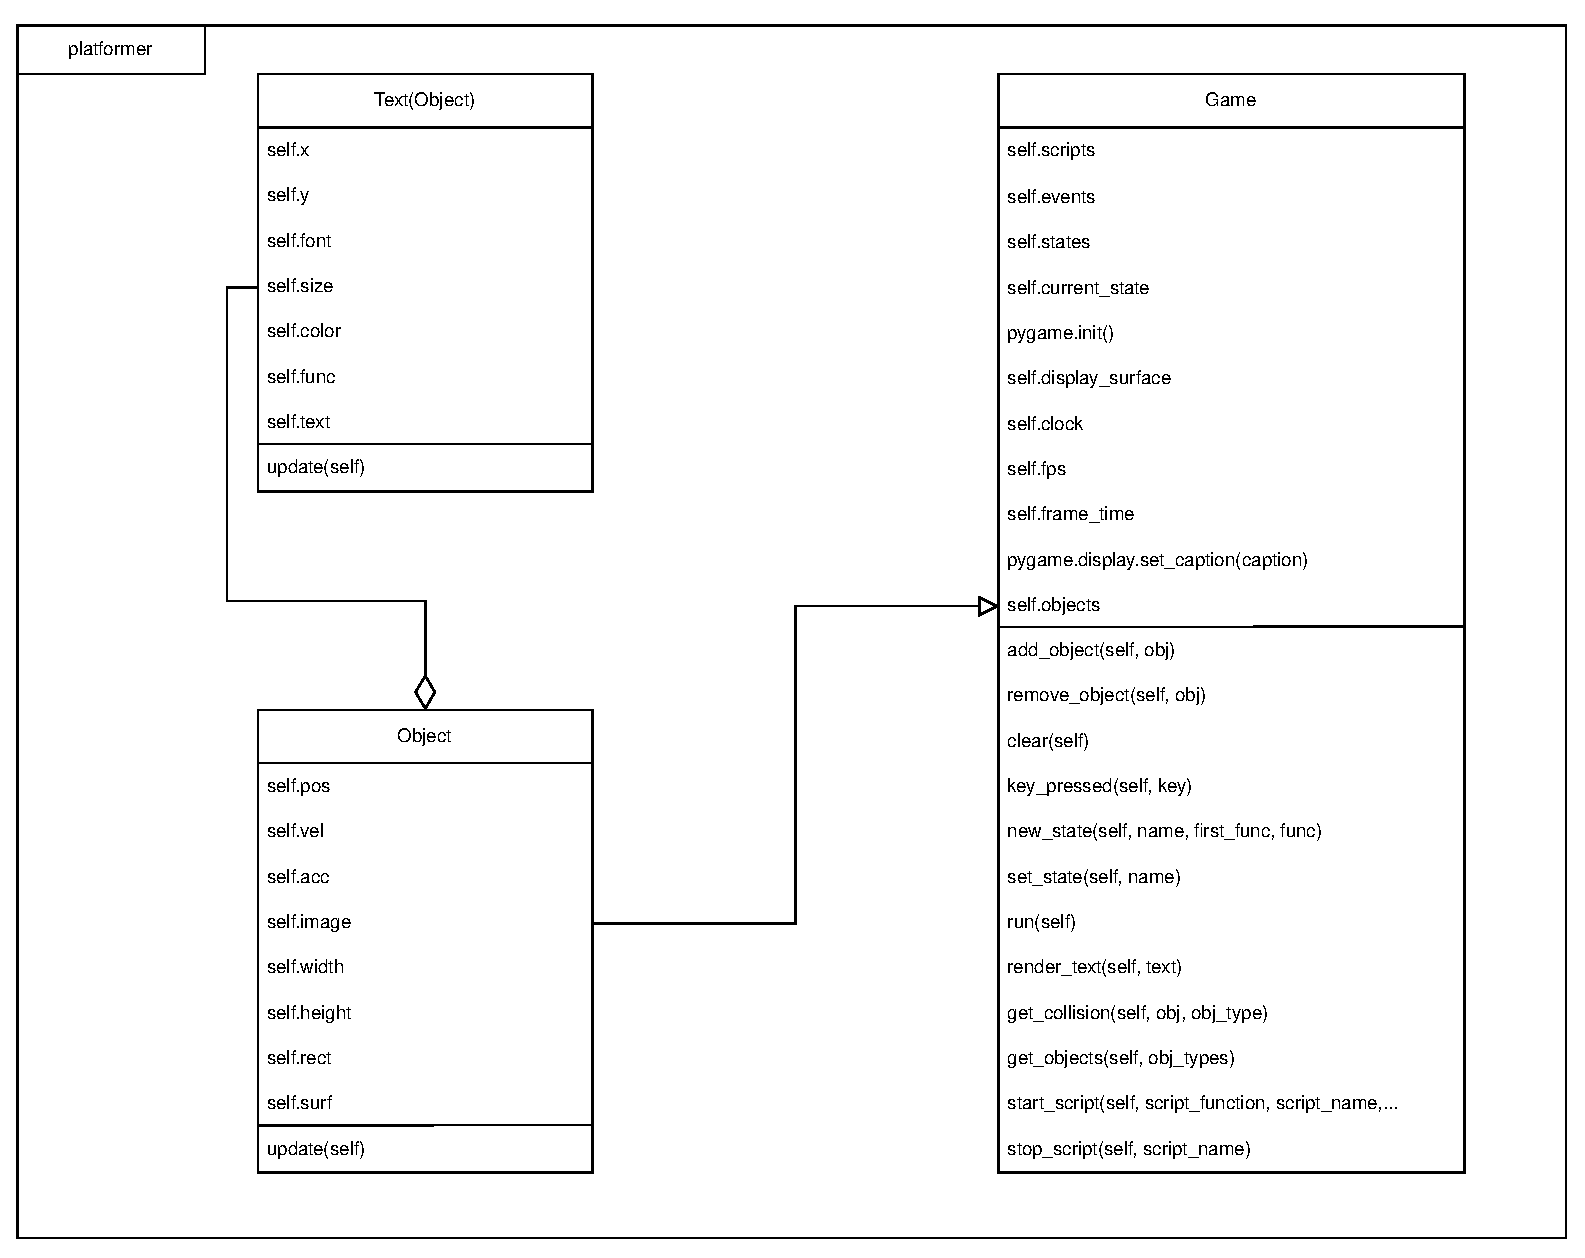
\includegraphics[width=1\linewidth]{platformer}}
	\caption{Диаграмма компонентов platformer}
	\label{platformer:image}
\end{figure}
\paragraph{Описание классов}
\begin{itemize}
		\item[Game] - класс системы платформера. Содержит в себе:
		\begin{enumerate}
				\item self.scripts - словарь для хранения запущенных сценариев;
				\item self.events - cловарь для хранения запущенных event`ов сценариев;
				\item self.states - словарь для хранения состояний игры;
				\item self.current\_state - текущее состояние;
				\item self.display\_surface - создание поверхности дисплея;
				\item self.clock - таймер;
				\item self.fps - количество ФПС(кадров в секунду);
				\item self.frame\_time - длительность кадра;
				\item self.objects.append(obj) - добавление объекта obj в игру;
				\item self.objects.remove(obj) - удаление объекта obj;
				\item self.objects - текущий список объектов;
				\item self.states[name] - создание нового игрового состояния;
				\item self.current\_state - текущее состояние;
				\item self.stop\_script остановка состояния;
				\item self.start\_script - запуск сценария;
				\item self.display\_surface.fill - заливка объекта сплошным цветом;
				\item self.render\_text - обработка текста;
				\item self.display\_surface.blit - отрисовка текстового объекта text;
				\item self.clock.tick - обновление таймера.
		\end{enumerate}
		\item[Object] - класс игрового объекта. Содержит в себе:
		\begin{enumerate}
				\item self.pos - координаты объекта;
				\item self.vel - скорость;
				\item self.acc - ускорение;
				\item self.image - изображение;
				\item self.width - ширина;
				\item self.height - высота;
				\item self.surf - объект для предоставления изображений;
				\item self.rect - прямоугольник;
				\item self.image.get\_width - ширина изображения;
				\item self.image.get\_height - высота изображения.
		\end{enumerate}
		\item[Text] - класс отвечающий за текст. Наследник класса Object. Содержит в себе:
		\begin{enumerate}
				\item self.x - координата x;
				\item self.y - координата y;
				\item self.font - имя шрифта;
				\item self.size - размер шрифта;
				\item self.color - цвет текста;
				\item self.func - функция получения строки текста для реактивного обновления;
				\item self.text - текст.
		\end{enumerate}
\end{itemize}		
Архитектура программы при использования многопоточности также может помочь в достижении более чистой архитектуры проекта. Большинство примеров, которые мы рассмотрим , не обязательно будут работать быстрее используя потоки. Но использование потоков поможет сделать их архитектуру чище и понятнее.
Потоки (Thread)
Стандартная библиотека Python предоставляет библиотеку threading, которая содержит необходимые классы для работы с потоками. Основной класс в этой библиотеки Thread. Чтобы запустить отдельный поток, нужно создать экземпляр потока Thread и затем запустить его с помощью метода .start(). Пример на рисунке \ref{treading:image}:
\begin{figure}[H]
	\begin{lstlisting}[language=Python]
		def start_script(self, script_function, script_name, *args):
			'''
			Запускает сценарий в отдельном потоке с возможностью остановки и передачи аргументов.
			
			:param: script_function: функция, содержащая код сценария
			:param: script_name: имя сценария
			:param: args: дополнительные аргументы, которые передаются в сценарий
			'''
			e = threading.Event()
			self.events[script_name] = e
			
			def func(e, args):
				while not e.is_set():
					script_function(*args)
					time.sleep(self.frame_time)
			
			script_thread = threading.Thread(target=func, args=(e, args))
			script_thread.daemon = True
			script_thread.start()
			self.scripts[script_name] = script_thread
		
		def stop_script(self, script_name):
			'''
			Останавливает сценарий по имени
			
			:param: script_name: имя сценария, который нужно остановить
			'''
			if script_name in self.scripts:
				self.events[script_name].set()
				del self.scripts[script_name]
				del self.events[script_name]
			else:
				# Если сценарий не существует
				print(f"Сценарий {script_name} не существует.")
	\end{lstlisting}  
	\caption{Пример метода tread.start}
	\label{treading:image}
\end{figure}
!!!Когда создается поток Thread, ему передается функцию и список, содержащий аргументы этой функции. В примере указывается Thread, чтобы он запустил функцию thread\_function() и передаем ему 1 в качестве аргумента.

Сама по себе функция thread\_function() мало что делает. Она просто выводит некоторые сообщения с промежутком time.sleep() между ними.
Демоны потоков.
В информатике daemon (демон) – это процесс, который работает в фоновом режиме.

Python потоки имеет особое значение для демонов. Демон потока (или как еще его можно назвать демонический поток) будет остановлен сразу после выхода из программы. Один из способов думать об этих определениях – считать демон потока как потоком, который работает в фоновом режиме, не беспокоясь о его завершении.

Если в программе запущены потоки, которые не являются демонами, то программа будет ожидать завершения этих потоков, прежде чем сможет завершится. Тем не менее, потоки, которые являются демонами, при закрытие программы просто убиваются, в каком бы они состояние ни находились.
join()
Чтобы указать одному потоку дождаться завершения другого потока, вам нужно вызывать .join().  Если вызвать .join(), этот оператор будет ждать, пока не завершится любой вид потока.

Диаграмма состояний ~\ref{State:image}.
\begin{figure}[H]
	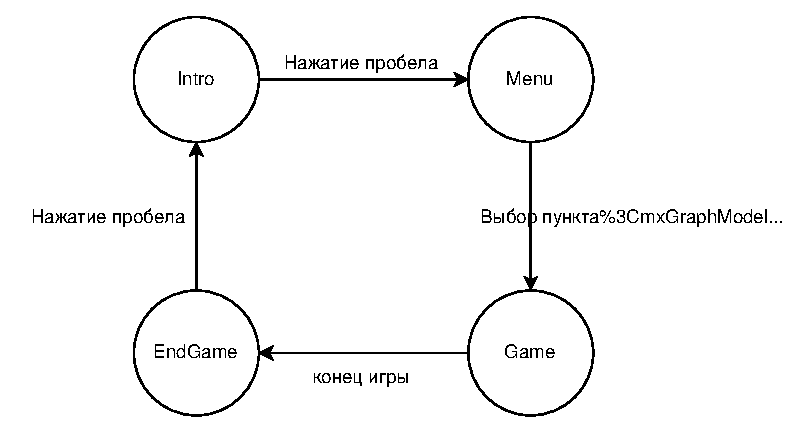
\includegraphics[width=1\linewidth]{State}
	\caption{Диаграмма состояний}
	\label{State:image}
\end{figure}

Диаграмма активности текущего состояния ~\ref{activestate:image}.
\begin{figure}[H]
	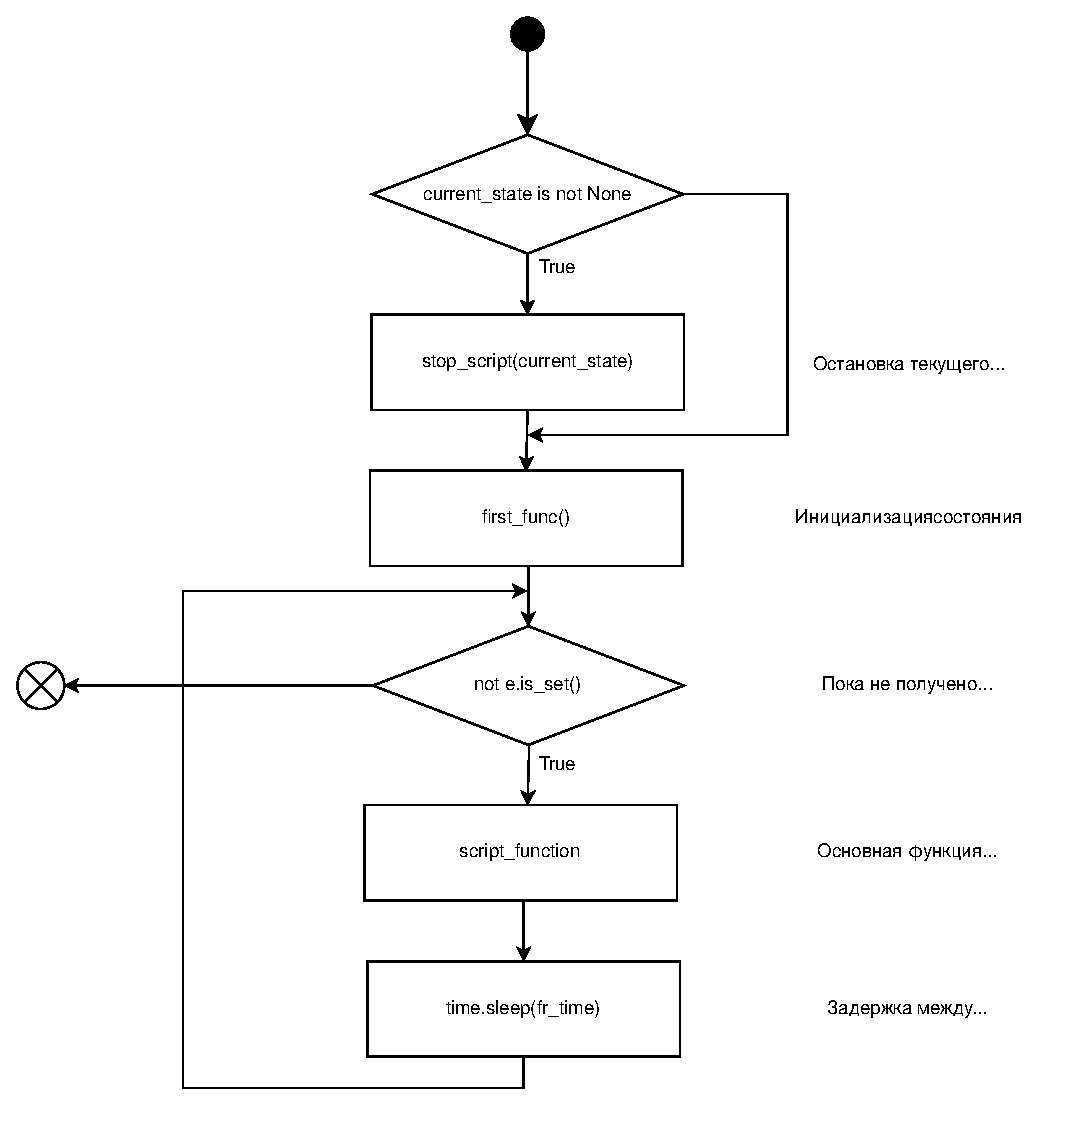
\includegraphics[width=1\linewidth]{activestate}
	\caption{Диаграмма активности текущего состояние}
	\label{activestate:image}
\end{figure}
		
				
\subsection{Пример диаграммы классов игры}

Диаграмма классов игры представлена на рисунке ~\ref{class:image}.
\begin{figure}[H]
	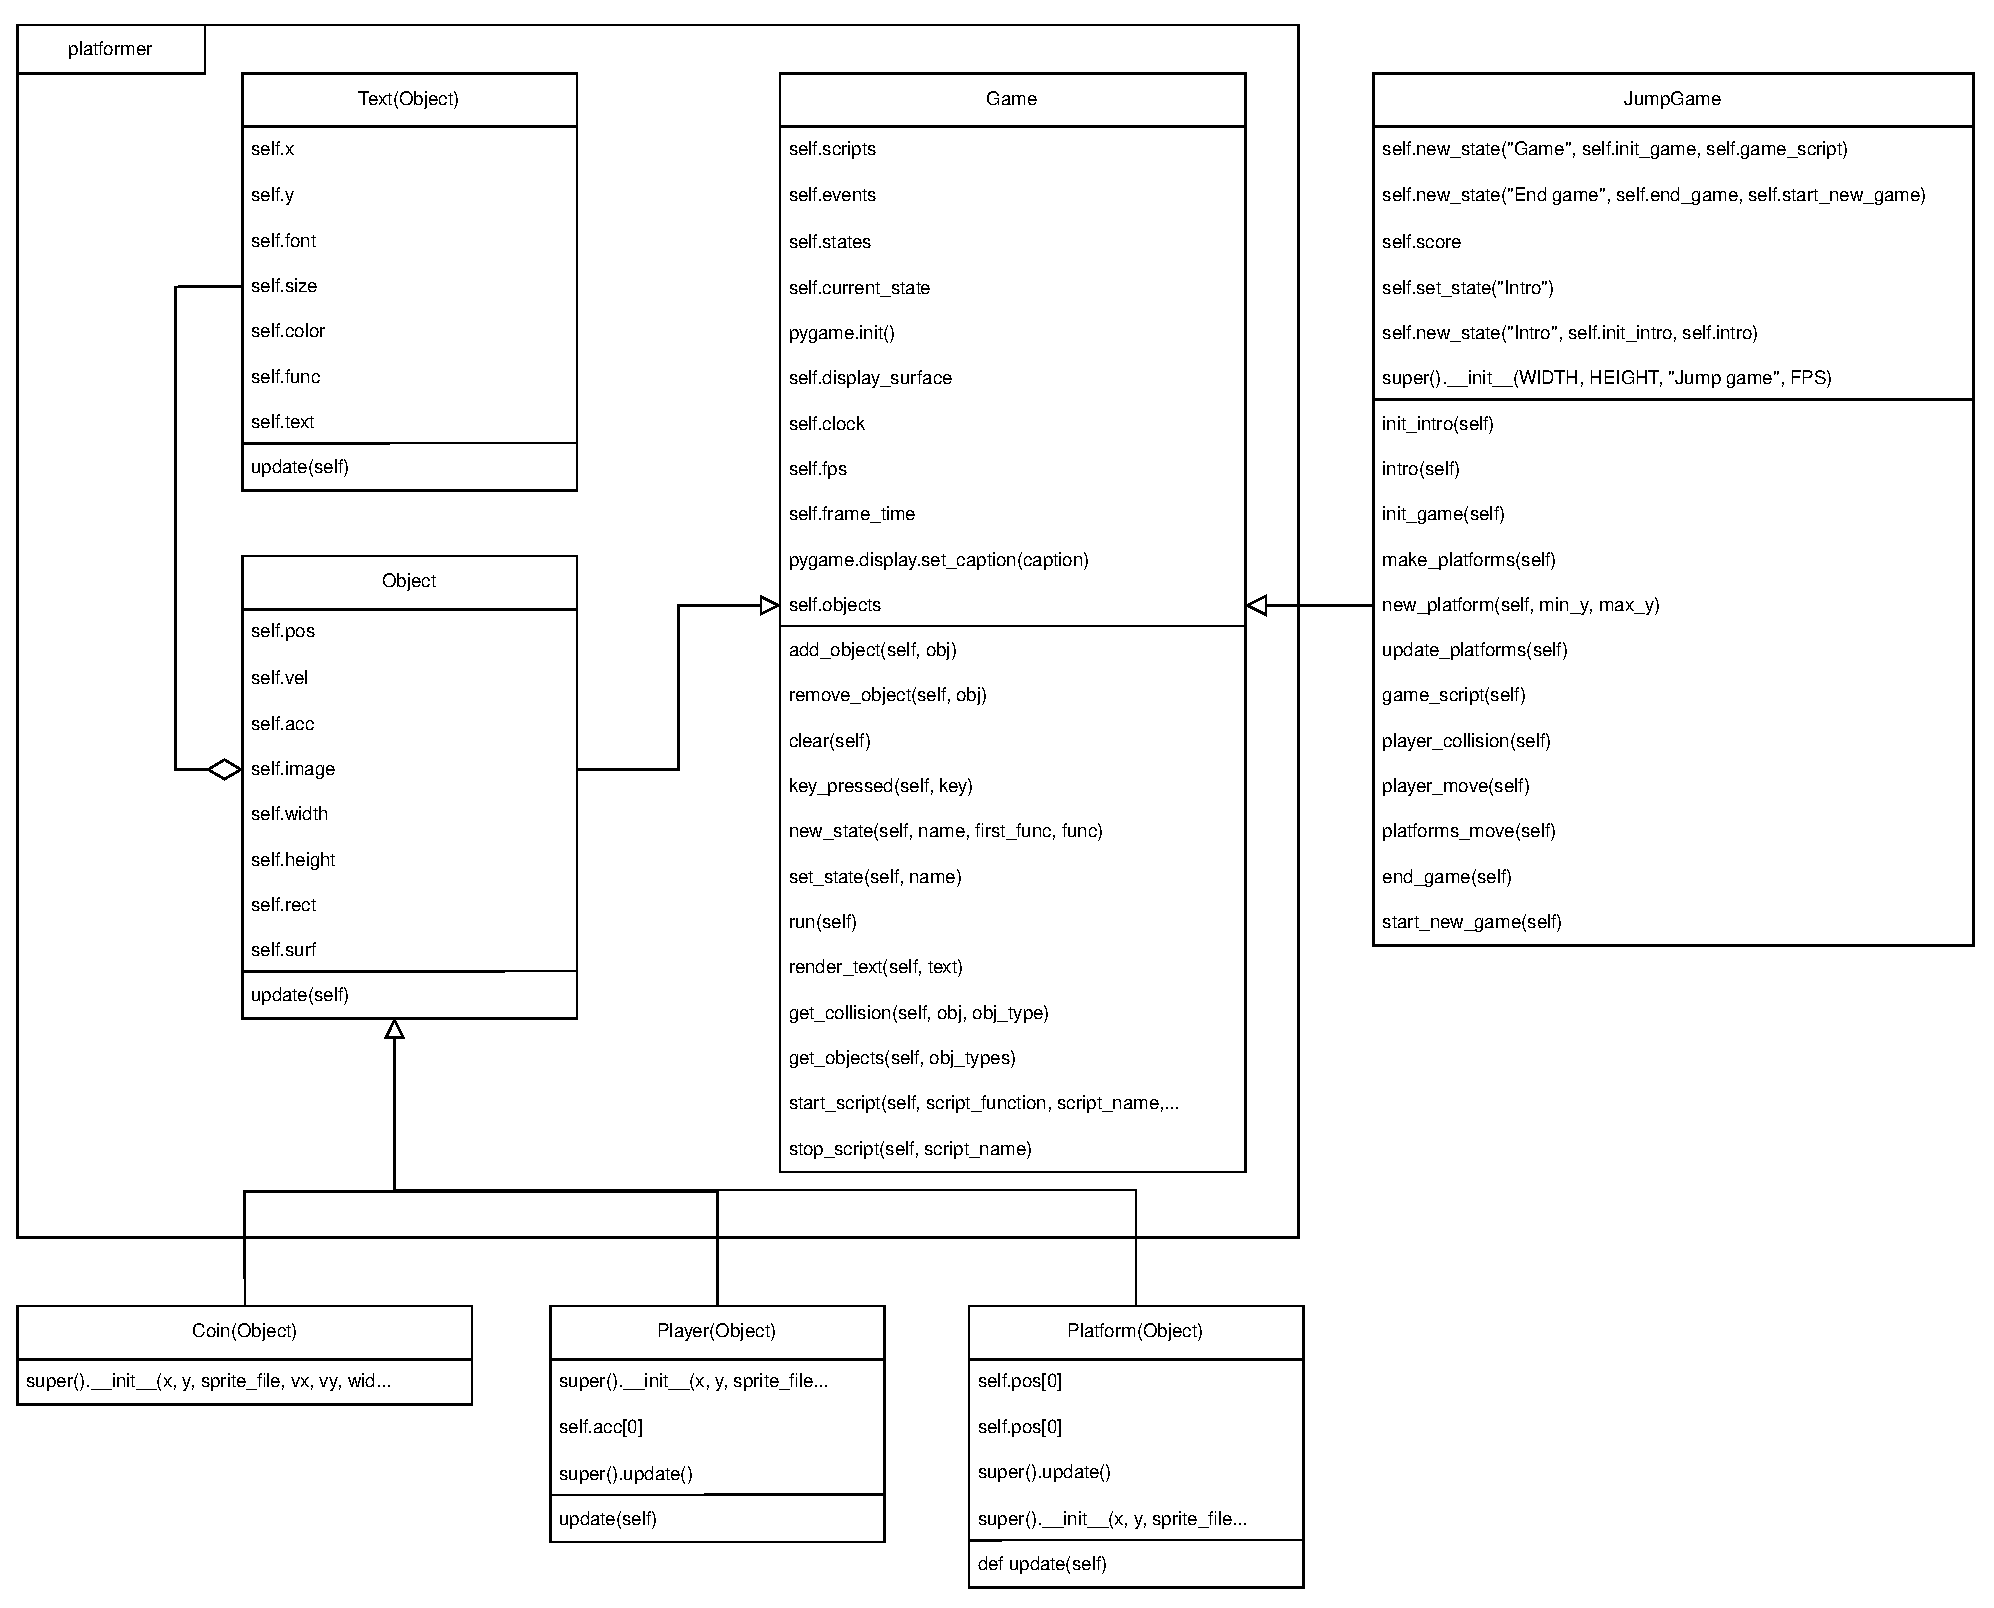
\includegraphics[width=1\linewidth]{class}
	\caption{Диаграмма классов игры}
	\label{class:image}
\end{figure}

 

\ifПрактика{}\else{
   \section{Рабочий проект}
\subsection{Классы, используемые при разработке сайта}

\subsubsection{Класс Game}

Класс Game относится к platformer и используется для управления программной системой.

Описание методов класса Game представлено в таблице \ref{table:game_methods}.
\renewcommand{\arraystretch}{0.8} % уменьшение расстояний до сетки таблицы
\begin{xltabular}{\textwidth}{|X|X|}
	\caption{Методы класса Game}\label{table:game_methods} \\
	\hline \centrow
	Название метода & \centrow  Описание метода \\
	\hline \centrow 1 & \centrow 2 \\ \hline
	\endfirsthead
	\continuecaption{Продолжение таблицы \ref{table:game_methods}}\\
	\hline \centrow 1 & \centrow 2 \\ \hline
	\finishhead
	add\_object(self, obj) & Добавляет объект obj в игру,параметр obj: добавляемый объект. \\
	\hline
	remove\_object(self, obj) & Удаляет объект obj из игры, параметр obj: удаляемый объект. \\
	\hline
	clear(self) & Удаляет все игровые объекты. \\
	\hline
	key\_pressed(self, key) & Возвращает True если была нажата клавиша key, иначе False, параметр key: нажимаемая кнопка. \\
	\hline
	new\_state(self, name, first\_func, func) & Создание нового игрового состояния, параметр name: имя состояния, параметр first\_func:функция, которая запускается при переключении в это игровое состояние, параметр func: функция, которая работает каждый кадр в этом игровом состянии. \\
	\hline
	set\_state(self, name) & Переключиться в игровое состояние, параметр name: имя состояния. \\
	\hline
	run(self) & Главный цикл игры. \\
	\hline
	render\_text(self, text) & Отрисовка текстового объекта, параметр text: текстовый объект. \\
	\hline
	get\_collision(self, obj, obj\_type) & Получение списка объектов столкновения, параметр obj: объект, с которым проверяется столкновение, параметр obj\_type:тип объектов, которые будут проверяться. \\
	\hline
	get\_objects(self, obj\_types) & Получение списка объектов заданного типа, параметр obj\_types: список требуемых типов. \\
	\hline
	start\_script(self, script\_function, script\_name, *args) & Запускает сценарий в отдельном потоке с возможностью остановки и передачи аргументов, параметр script\_function: функция, содержащая код сценария, параметр script\_name: имя сценария, параметр args: дополнительные аргументы, которые передаются в сценарий. \\
	\hline
	stop\_script(self, script\_name) & Останавливает сценарий по имени, параметр script\_name: имя сценария, который нужно остановить. \\
	\hline
\end{xltabular}

\subsubsection{Класс Object}

Класс Object относится к platformer, является классом игровых объектов и предназначен для создания, обновления и работы с игровыми объектами.

Описание методов класса Object представлено в таблице \ref{table:object_methods}.

\begin{xltabular}{\textwidth}{|X|X|}
	\caption{Методы класса Object}\label{table:object_methods} \\
	\hline \centrow
	Название метода & \centrow  Описание метода \\
	\hline \centrow 1 & \centrow 2 \\ \hline
	\endfirsthead
	\continuecaption{Продолжение таблицы \ref{table:object_methods}}\\
	\hline \centrow 1 & \centrow 2 \\ \hline
	\finishhead
	update(self) & Обновляет состояние объекта каждый кадр. \\
	\hline
\end{xltabular}

\subsubsection{Класс Text(Object)}

Класс Text(Object) относится к platformer, является наследником класса Object, используется для работы с текстовыми объектами(создание и обновление текстовой строки).

Описание методов класса Text(Object) представлено в таблице \ref{table:text_methods}.

\begin{xltabular}{\textwidth}{|X|X|}
	\caption{Методы класса Text(Object)}\label{table:text_methods} \\
	\hline \centrow
	Название метода & \centrow  Описание метода \\
	\hline \centrow 1 & \centrow 2 \\ \hline
	\endfirsthead
	\continuecaption{Продолжение таблицы \ref{table:text_methods}}\\
	\hline \centrow 1 & \centrow 2 \\ \hline
	\finishhead
	update(self) & Обновляет текст из функции. \\
	\hline
\end{xltabular}

\subsubsection{Класс Player(Object)}

Класс Player(Object) - это класс игрока, является наследником класса Object.

Описание методов класса Player(Object) представлено в таблице \ref{table:player_methods}.

\begin{xltabular}{\textwidth}{|X|X|}
	\caption{Методы класса Player(Object)}\label{table:player_methods} \\
	\hline \centrow
	Название метода & \centrow  Описание метода \\
	\hline \centrow 1 & \centrow 2 \\ \hline
	\endfirsthead
	\continuecaption{Продолжение таблицы \ref{table:player_methods}}\\
	\hline \centrow 1 & \centrow 2 \\ \hline
	\finishhead
	update(self) & обновление состояния игрока. \\
	\hline
\end{xltabular}

\subsubsection{Класс Platform(Object)}

Класс Platform(Object) - это класс игровых платформ, является наследником класса Object.

Описание методов класса Platform(Object) представлено в таблице \ref{table:platform_methods}.

\begin{xltabular}{\textwidth}{|X|X|}
	\caption{Методы класса Platform(Object)}\label{table:platform_methods} \\
	\hline \centrow
	Название метода & \centrow  Описание метода \\
	\hline \centrow 1 & \centrow 2 \\ \hline
	\endfirsthead
	\continuecaption{Продолжение таблицы \ref{table:platform_methods}}\\
	\hline \centrow 1 & \centrow 2 \\ \hline
	\finishhead
	update(self) & обновление состояния платформ. \\
	\hline
\end{xltabular}

\subsubsection{Класс Coin(Object)}

Класс Coin(Object) - это класс собираемых объектов(монеток), является наследником класса Object.

Описание методов класса Coin(Object) представлено в таблице \ref{table:coin_methods}.

\begin{xltabular}{\textwidth}{|X|X|}
	\caption{Методы класса Coin(Object)}\label{table:coin_methods} \\
	\hline \centrow
	Название метода & \centrow  Описание метода \\
	\hline \centrow 1 & \centrow 2 \\ \hline
	\endfirsthead
	\continuecaption{Продолжение таблицы \ref{table:coin_methods}}\\
	\hline \centrow 1 & \centrow 2 \\ \hline
	\finishhead
	 \_\_init\_\_(self, x, y, sprite\_file, vx=0, vy=0, width=None, height=None) & Инициализирует класс Coin, параметр:x, координата x, параметр:y, координата y, параметр:sprite\_file, файл изображения, параметр:vx, скорость по координате x, параметр:vy, скорость по координате y, параметр:width, ширина, параметр:height, высота. \\
	\hline
\end{xltabular}

\subsubsection{Класс JumpGame(Game)}

Класс JumpGame(Game) является наследником класса Game и представляет из себя игру демонстрирующую работу нашей программной системы.

Описание методов класса JumpGame(Game) представлено в таблице \ref{table:jumpgame_methods}.
\renewcommand{\arraystretch}{0.8} % уменьшение расстояний до сетки таблицы
\begin{xltabular}{\textwidth}{|X|X|}
	\caption{Методы класса JumpGame(Game)}\label{table:jumpgame_methods} \\
	\hline \centrow
	Название метода & \centrow  Описание метода \\
	\hline \centrow 1 & \centrow 2 \\ \hline
	\endfirsthead
	\continuecaption{Продолжение таблицы \ref{table:jumpgame_methods}}\\
	\hline \centrow 1 & \centrow 2 \\ \hline
	\finishhead
	init\_intro(self) & Представляет из себя начало заставки. \\
	\hline
	intro(self) & Представляет из себя сценарий заставки. \\
	\hline
	init\_game(self) & Запуск начала игры. \\
	\hline
	make\_platforms(self) & Генерирует начальные платформы. \\
	\hline
	new\_platform(self, min\_y, max\_y) & Создание новой платформы с монеткой, параметр min\_y: минимальная координата платформы, параметр max\_y:максимальная координата платформы. \\
	\hline
	update\_platforms(self) & Генерация дополнительных платформ, чтобы их число было равно заданному. \\
	\hline
	game\_script(self) & Сценарий игры, выполняемый каждый кадр. \\
	\hline
	player\_collision(self) & Представляет из себя логику столкновений игрока с объектами игры. \\
	\hline
	player\_move(self) & Представляет из себя логику движения игрока. \\
	\hline
	platforms\_move(self) & Перемещение платформ с монетами вниз, когда игрок перемещается вверх. \\
	\hline
	end\_game(self) & Оповещение о смерти персонажа и конце игры. \\
	\hline
	start\_new\_game(self) & Запускает новую игру, переход на intro. \\
	\hline
\end{xltabular}

\subsection{Системное тестирование разработанного приложения}

На рисунке \ref{Intro_systemtest:image} представлен пример состояния "Intro" при запуске программы.
\begin{figure}[H]
	\centering
	
\includegraphics[width=1\linewidth]{Intro_systemtest}
	\caption{Состояние "Intro" при запуске программы}
	\label{Intro_systemtest:image}
\end{figure}

На рисунке \ref{spawn:image} представлен пример начальной позиции игрока(начальное состояние игры).
\begin{figure}[H]
	\centering
	
\includegraphics[width=1\linewidth]{spawn}
	\caption{Начало игры}
	\label{spawn:image}
\end{figure}

На рисунке \ref{PlatPoint:image} представлено начисление 1 очка за прыжок на новую платформу.
\begin{figure}[H]
	\centering
	
\includegraphics[width=1\linewidth]{PlatPoint}
	\caption{Начисление очков за передвижение по платформам}
	\label{PlatPoint:image}
\end{figure}

На рисунке \ref{TakeCoin:image} представлен пример начисления 5 очков за сбор монетки.
\begin{figure}[H]
	\centering
	
\includegraphics[width=1\linewidth]{TakeCoin}
	\caption{Начисление очков за сбор монеток}
	\label{TakeCoin:image}
\end{figure}

На рисунке \ref{SixPlat:image} представлена постоянная отрисовка 6 платформ.В примере персонаж стоит на платформе 1 и прыгает на платформу 3, после этого платформы 4,5,6 находившиеся снизу ушли за экран, были удалены, а сверху появились новые платформы 4,5,6.
\begin{figure}[H]
	\centering
	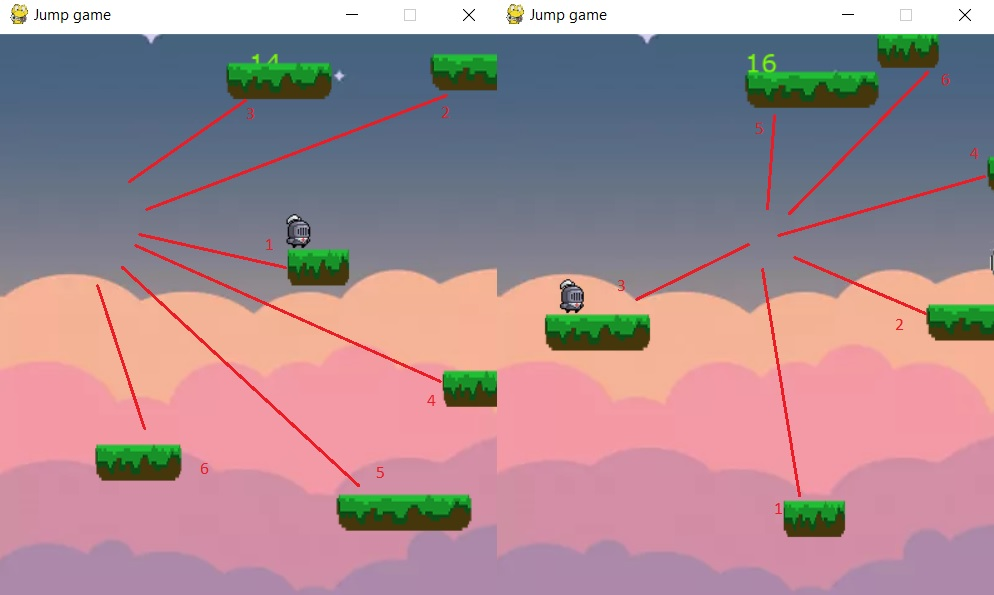
\includegraphics[width=1\linewidth]{SixPlat}
	\caption{Пример постоянной отрисовки 6 платформ}
	\label{SixPlat:image}
\end{figure}

На рисунке \ref{Death:image} представлен пример работы сценария "End Game".
\begin{figure}[H]
	\centering
	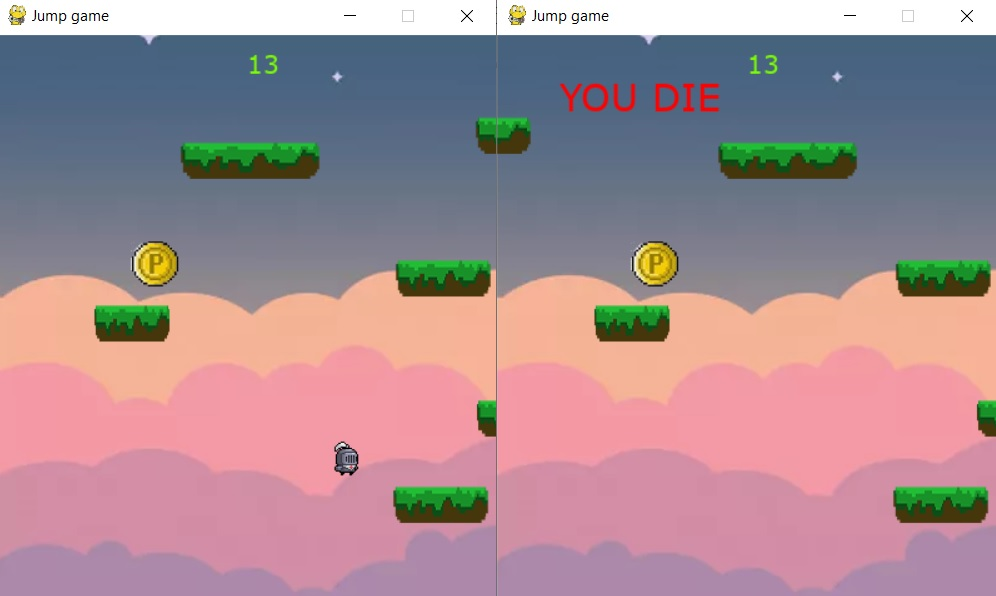
\includegraphics[width=1\linewidth]{Death}
	\caption{Пример работы сценария "End Game"}
	\label{Death:image}
\end{figure}

На рисунке \ref{DeathIntro:image} представлен пример работы смены сценария "End Game" на сценарий "Intro".
\begin{figure}[H]
	\centering
	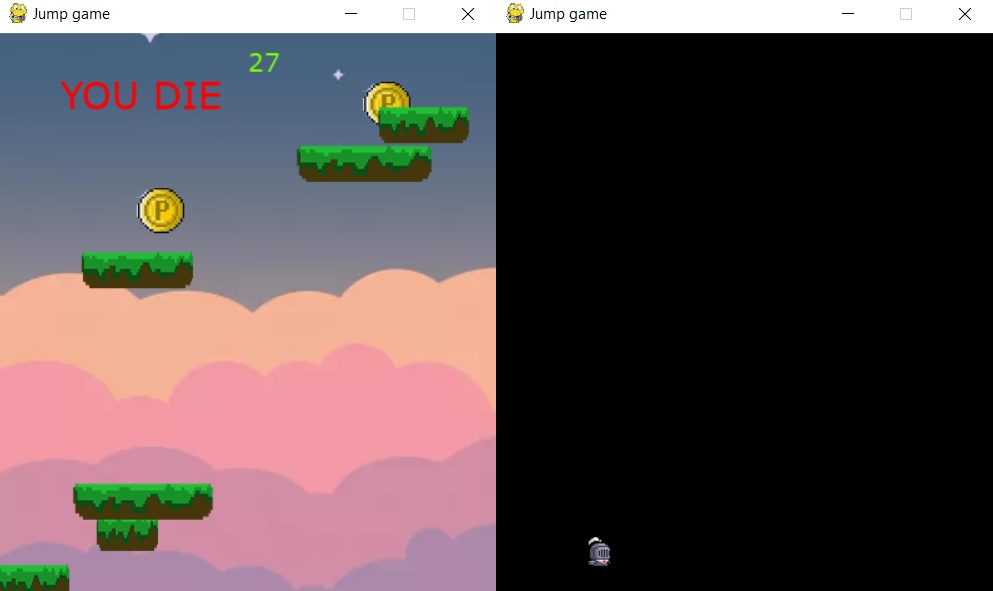
\includegraphics[width=1\linewidth]{DeathIntro}
	\caption{Пример смены сценариев}
	\label{DeathIntro:image}
\end{figure}


   \section*{ЗАКЛЮЧЕНИЕ}
\addcontentsline{toc}{section}{ЗАКЛЮЧЕНИЕ}

В заключение, программная система для создания игр-платформеров с заранее отрисованным двумерным фоном и спрайтовыми персонажами представляет собой мощный инструмент, который открывает широкие возможности для разработчиков и дизайнеров. Она позволяет воплощать в жизнь уникальные игровые миры с богатой графикой и детализированными персонажами, сохраняя при этом ощущение ностальгии по временам когда этот жанр был наиболее популярен. Эта программная система не только упрощает процесс разработки игр, но и делает его более доступным для широкого круга творческих людей, желающих реализовать свои идеи без необходимости владения сложными навыками программирования. Таким образом, она способствует росту индустрии компьютерных игр и обогащает культурное пространство новыми, захватывающими проектами.

Основные результаты работы:

\begin{enumerate}
	\item Проведен анализ предметной области.
	\item Разработана концептуальная модель приложения. Разработана модель данных системы. Определены требования к системе.
	\item Осуществлено проектирование приложения. Разработан пользовательский интерфейс приложения.
	\item Реализовано и протестировано приложение. Проведено модульное и системное тестирование.
\end{enumerate}

Все требования, объявленные в техническом задании, были полностью реализованы, все задачи, поставленные в начале разработки проекта, были также решены.
}\fi
\addcontentsline{toc}{section}{СПИСОК ИСПОЛЬЗОВАННЫХ ИСТОЧНИКОВ}

\begin{thebibliography}{9}

    \bibitem{javascript} Фримен, А. Практикум по программированию на JavaScript / А. Фримен. – Москва~: Вильямс, 2013. – 960 с. – ISBN 978-5-8459-1799-7. – Текст~: непосредственный.
    \bibitem{php} Бретт, М. PHP и MySQL. Исчерпывающее руководство / М. Бретт. – Санкт-Петербург : Питер, 2016. – 544 с. – ISBN 978-5-496-01049-8. – Текст~: непосредственный.
    \bibitem{css} Веру, Л. Секреты CSS. Идеальные решения ежедневных задач / Л. Веру. – Санкт-Петербург : Питер, 2016. – 336 с. – ISBN 978-5-496-02082-4. – Текст~: непосредственный.
    \bibitem{mysql}	Гизберт, Д. PHP и MySQL / Д. Гизберт. – Москва~: НТ Пресс, 2013. – 320 с. – ISBN 978-5-477-01174-2. – Текст~: непосредственный.
	\bibitem{html5}	Голдстайн, А. HTML5 и CSS3 для всех / А. Голдстайн, Л. Лазарис, Э. Уэйл. – Москва~: Вильямс, 2012. – 368 с. – ISBN 978-5-699-57580-0. – Текст~: непосредственный.
	\bibitem{htmlcss}	Дэкетт, Д. HTML и CSS. Разработка и создание веб-сайтов / Д. Дэкетт. – Москва~: Эксмо, 2014. – 480 с. – ISBN 978-5-699-64193-2. – Текст~: непосредственный.
	\bibitem{bigbook}	Макфарланд, Д. Большая книга CSS / Д. Макфарланд. – Санкт-Петербург : Питер, 2012. – 560 с. – ISBN 978-5-496-02080-0. – Текст~: непосредственный.
	\bibitem{uchiru}	Лоусон, Б. Изучаем HTML5. Библиотека специалиста / Б. Лоусон, Р. Шарп. – Санкт-Петербург : Питер, 2013 – 286 с. – ISBN 978-5-459-01156-2. – Текст~: непосредственный.
	\bibitem{chaynik}	Титтел, Э. HTML5 и CSS3 для чайников / Э. Титтел, К. Минник. – Москва~: Вильямс, 2016 – 400 с. – ISBN 978-1-118-65720-1. – Текст~: непосредственный.    
	\bibitem{22}	Титтел, Э. HTML5 и CSS3 для чайников / Э. Титтел, К. Минник. – Москва~: Вильямс, 2016 – 400 с. – ISBN 978-1-118-65720-1. – Текст~: непосредственный.    
	\bibitem{1231}	Титтел, Э. HTML5 и CSS3 для чайников / Э. Титтел, К. Минник. – Москва~: Вильямс, 2016 – 400 с. – ISBN 978-1-118-65720-1. – Текст~: непосредственный.    
	\bibitem{sdf}	Титтел, Э. HTML5 и CSS3 для чайников / Э. Титтел, К. Минник. – Москва~: Вильямс, 2016 – 400 с. – ISBN 978-1-118-65720-1. – Текст~: непосредственный.    
	\bibitem{servsssds}	Титтел, Э. HTML5 и CSS3 для чайников / Э. Титтел, К. Минник. – Москва~: Вильямс, 2016 – 400 с. – ISBN 978-1-118-65720-1. – Текст~: непосредственный.
\end{thebibliography}

\ifВКР{\appendix{Представление графического материала}

Графический материал, выполненный на отдельных листах,
изображен на рисунках А.1--А.\arabic{числоПлакатов}.
\setcounter{числоПлакатов}{0}

\renewcommand{\thefigure}{А.\arabic{figure}} % шаблон номера для плакатов

\begin{landscape}

\begin{плакат}
    
\includegraphics[width=0.82\linewidth]{плакат1.png}
    \заголовок{Сведения о ВКРБ}
    \label{pl1:image}      
\end{плакат}

\begin{плакат}
    
\includegraphics[width=0.82\linewidth]{плакат2.png}
    \заголовок{Цель и задачи разработки}
    \label{pl2:image}      
\end{плакат}

\begin{плакат}
    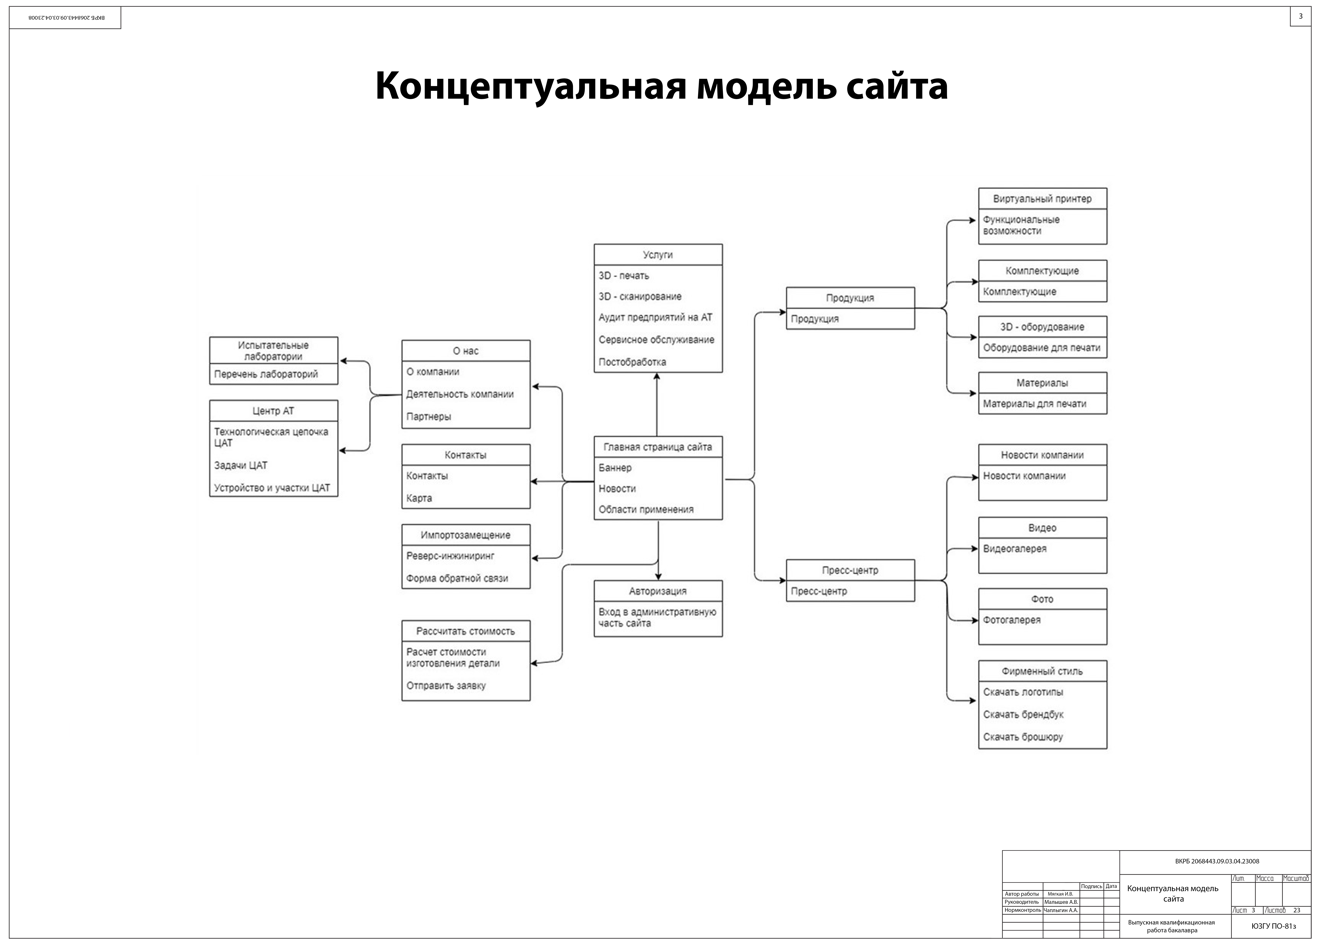
\includegraphics[width=0.82\linewidth]{плакат3.png}
    \заголовок{Концептуальная модель сайта}
    \label{pl3:image}      
\end{плакат}

\begin{плакат}
    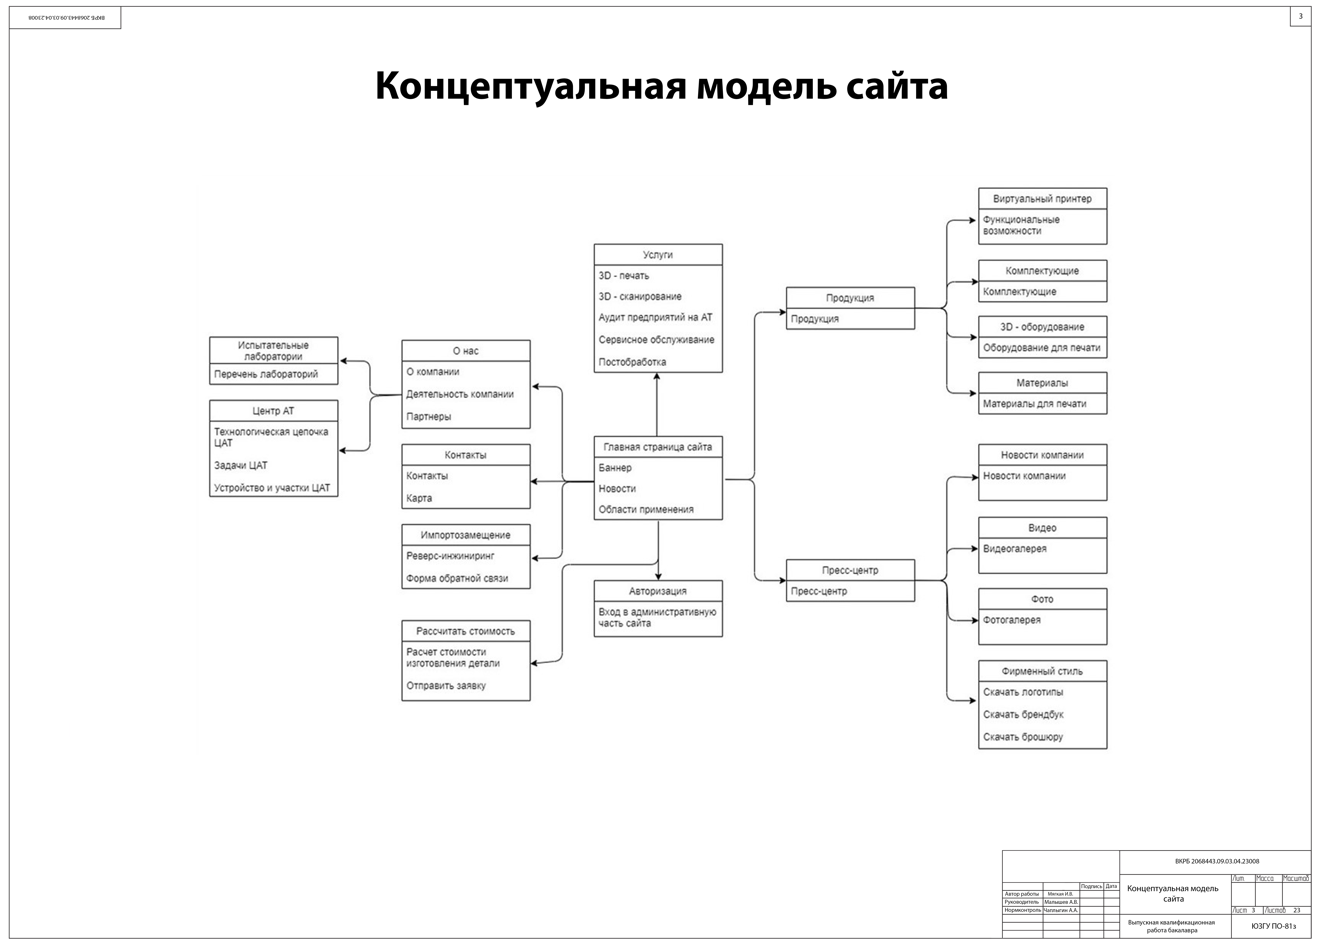
\includegraphics[width=0.82\linewidth]{плакат3.png}
    \заголовок{Еще плакат}
    \label{pl4:image}      
\end{плакат}

\end{landscape}
}\fi
\ifПрактика{}\else{\appendix{Фрагменты исходного кода программы}

main.tex
\lstinputlisting[language=Tex, frame=none]{main.tex}

ТехПроект.tex
\lstinputlisting[language=Tex, frame=none]{ТехПроект.tex}

\ifВКР{
\newpage
\addcontentsline{toc}{section}{На отдельных листах (CD-RW в прикрепленном конверте)}
\begin{center}
\textbf{Место для диска}
\end{center}
}\fi
}\fi
\end{document}
